% -*- latex -*-
%%%%%%%%%%%%%%%%%%%%%%%%%%%%%%%%%%%%%%%%%%%%%%%%%%%%%%%%%%%%%%%%
%%%%%%%%%%%%%%%%%%%%%%%%%%%%%%%%%%%%%%%%%%%%%%%%%%%%%%%%%%%%%%%%
%%%%
%%%% This text file is part of the source of 
%%%% `Parallel Programming in MPI and OpenMP'
%%%% by Victor Eijkhout, copyright 2012-2021
%%%%
%%%% mpi-nonblock.tex : blocking sends
%%%%
%%%%%%%%%%%%%%%%%%%%%%%%%%%%%%%%%%%%%%%%%%%%%%%%%%%%%%%%%%%%%%%%
%%%%%%%%%%%%%%%%%%%%%%%%%%%%%%%%%%%%%%%%%%%%%%%%%%%%%%%%%%%%%%%%

\Level 0 {Nonblocking point-to-point operations}
\label{sec:nonblock}

The structure of communication is often a reflection of the structure
of the operation.
With some regular applications we also get a regular communication pattern.
Consider again the above operation:
\[ y_i=x_{i-1}+x_i+x_{i+1}\colon i=1,\ldots,N-1 \]
Doing this in parallel induces communication, as pictured in figure~\ref{fig:3pt-interior}.

%% \begin{figure}[ht]
%%   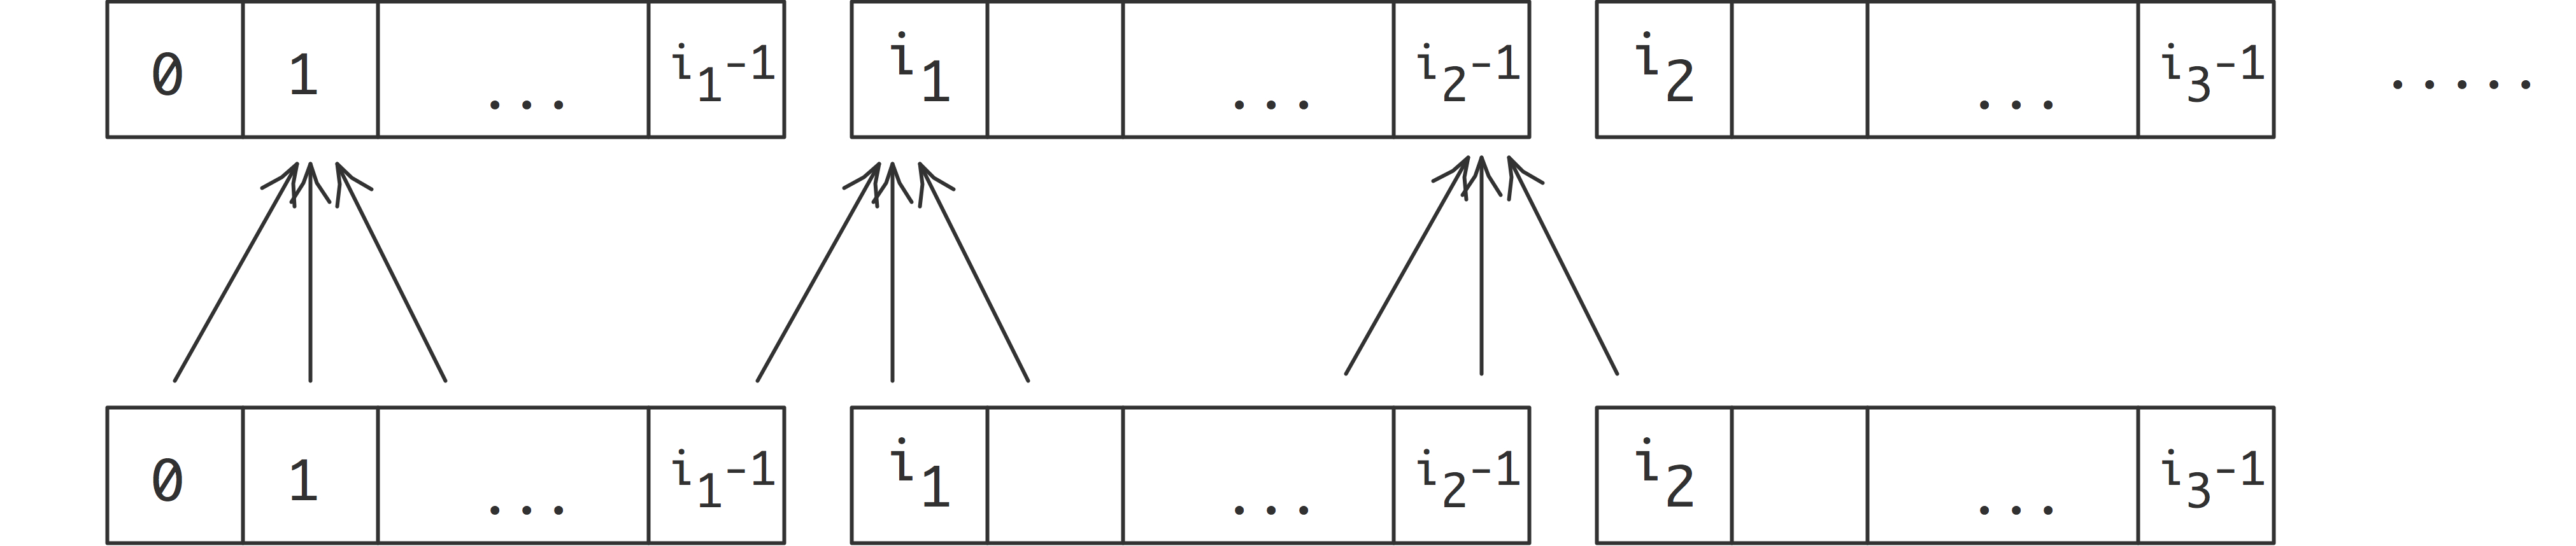
\includegraphics[scale=.09]{threepoint}
%%   \caption{Communication in an one-dimensional operation}
%%   \label{fig:3pt}
%% \end{figure}

We note:
\begin{itemize}
\item The data is one-dimensional, and we have a linear ordering of the processors.
\item The operation involves neighboring data points, and we communicate
  with neighboring processors.
\end{itemize}

Above you saw how you can use information exchange between pairs of processors
\begin{itemize}
\item using \indexmpishow{MPI_Send} and \indexmpishow{MPI_Recv}, if you are careful; or
\item using \indexmpishow{MPI_Sendrecv}, as long as there is indeed some sort of pairing of processors.
\end{itemize}
However, there are circumstances where it is not possible, not efficient, or simply not
convenient, to have such a deterministic setup of the send and receive calls.
%
\begin{figure}[ht]
  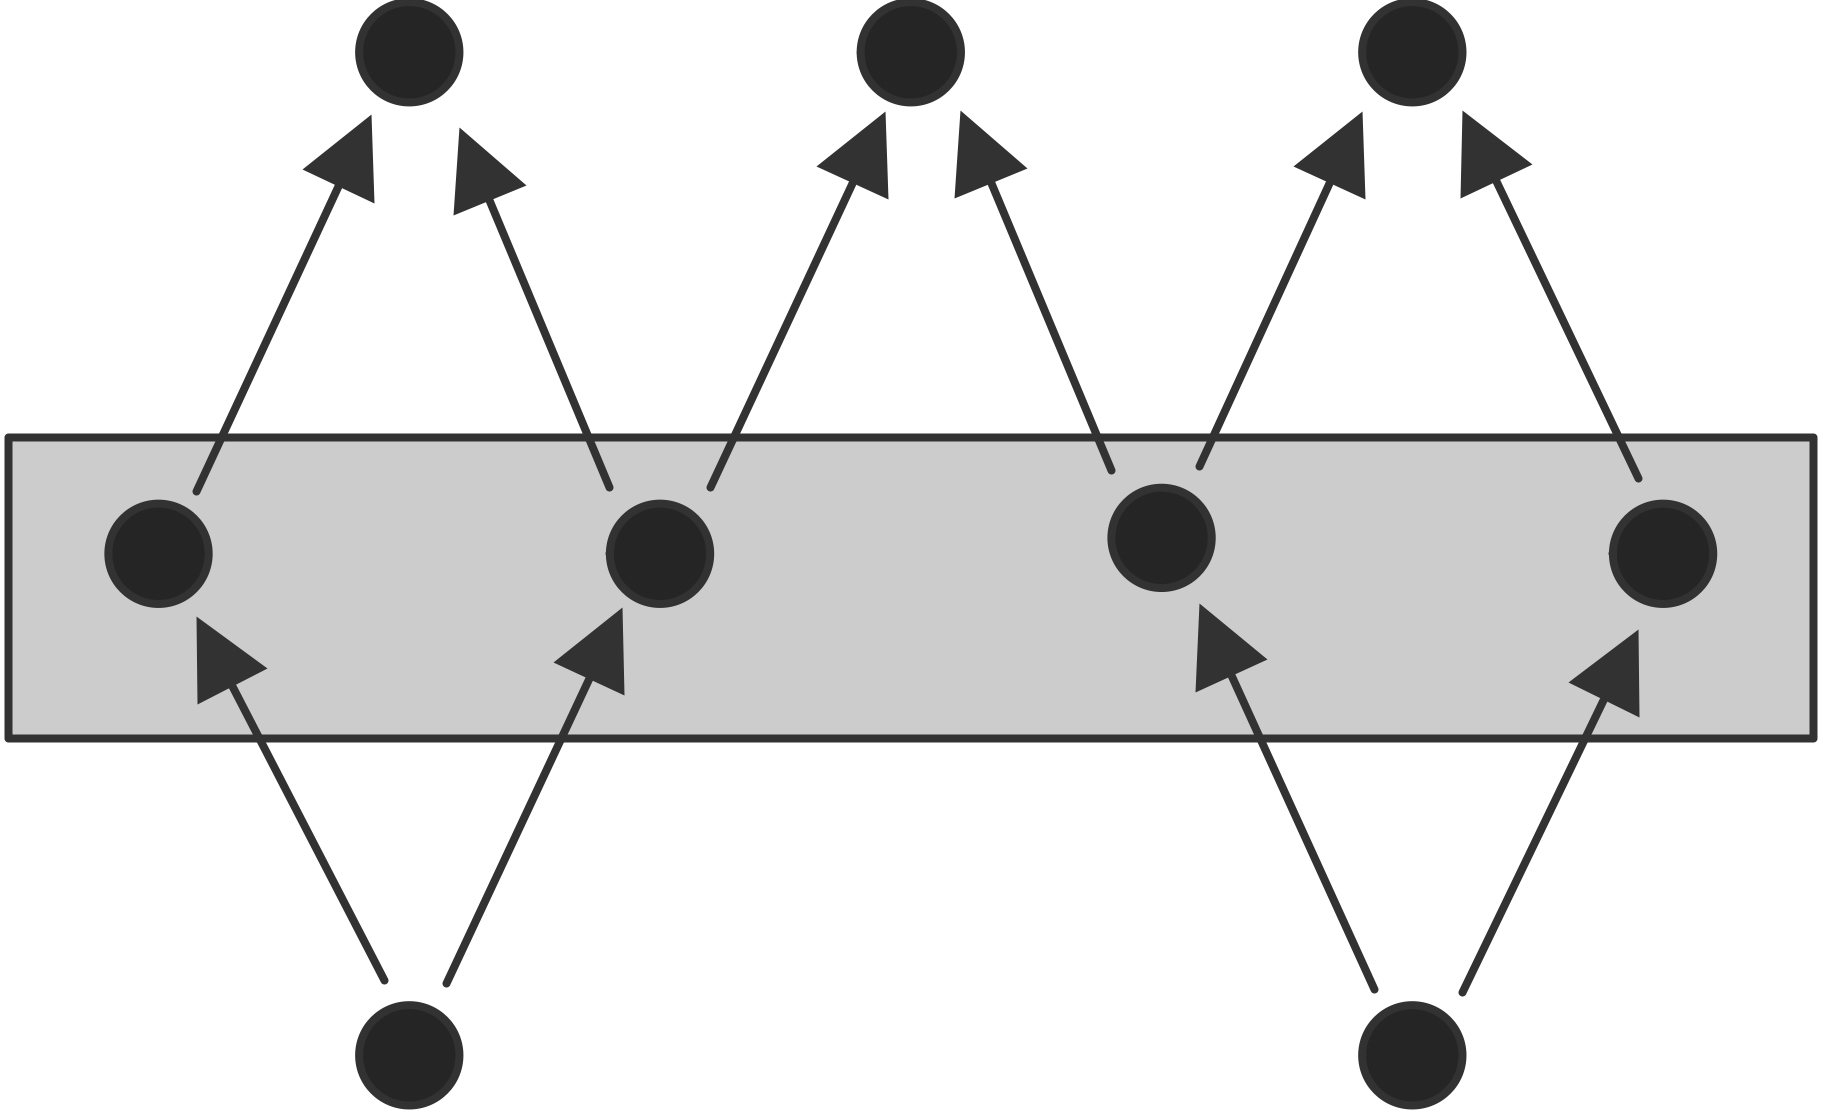
\includegraphics[scale=.1]{graphsend}
  \caption{Processors with unbalanced send/receive patterns}
  \label{fig:graphsend}
\end{figure}
%
Figure~\ref{fig:graphsend} illustrates such a case, where processors are
organized in a general graph pattern. Here, the numbers of sends and receive
of a processor do not need to match.

In such cases, one wants a possibility to state `these are the expected incoming
messages', without having to wait for them in sequence. Likewise, one wants to declare
the outgoing messages without having to do them in any particular sequence.
Imposing any sequence on the sends and receives is likely to run into the serialization
behavior observed above, or at least be inefficient.

\Level 1 {Nonblocking send and receive calls}
\label{sec:nonblocking}
\index{communication!nonblocking|(textbf}

In the previous section you saw that blocking communication makes
programming tricky if you want to avoid \indexterm{deadlock} and performance
problems. The main advantage of these routines is that you have full
control about where the data is: if the send call returns
the data has been successfully received, and the send buffer can be used for
other purposes or de-allocated.  

\begin{figure}[ht]
  \includegraphics[scale=.1]{send-nonblocking}
  \caption{Nonblocking send}
  \label{fig:send-nonblocking}
\end{figure}

By contrast, the nonblocking calls
\indexmpiref{MPI_Isend} and \indexmpiref{MPI_Irecv}
(where the `I' stands for
`\emph{immediate}'\index{immediate operation}
or
`\emph{incomplete}'\index{incomplete operation|see{operation, incomplete}}
)
do not wait for their counterpart: in effect
they tell the runtime system `here is some data and please send it as
follows' or `here is some buffer space, and expect such-and-such data
to come'.  This is illustrated in figure~\ref{fig:send-nonblocking}.
%
\cverbatimsnippet[examples/mpi/c/isendandirecv.c]{isendexample}
\cverbatimsnippet[examples/mpi/c/isendandirecv.c]{irecvexample}
%
Issuing the \indexmpishow{MPI_Isend}~/ \indexmpishow{MPI_Irecv}
call is sometimes referred to as
\emph{posting}\index{posting!of send/receive}
a send/receive.

\Level 1 {Request completion: wait calls}
\label{sec:waittest}

From the definition of \indexmpishow{MPI_Isend}~/
\indexmpishow{MPI_Irecv}, you seen that nonblocking routine yields
an \indexmpidef{MPI_Request} object. This request can then be used to
query whether the operation has concluded. You may also notice that
the \indexmpishow{MPI_Irecv} routine does not yield an
\indexmpishow{MPI_Status} object.  This makes sense: the status object
describes the actually received data, and at the completion of the
\indexmpishow{MPI_Irecv} call there is no received data yet.

Waiting for the request is done with a number of routines. We first
consider \indexmpiref{MPI_Wait}. It takes the request as input, and
gives an \indexmpishow{MPI_Status} as output. If you don't need the
status object, you can pass \indexmpishow{MPI_STATUS_IGNORE}.

\cverbatimsnippet[examples/mpi/c/hangwait.c]{bcastsendwait}

(Note that this example uses a mix of blocking and non-blocking
operations: a blocking send is paired with a non-blocking receive.)

The request is passed by reference, so that the wait routine
can free it:
\begin{itemize}
\item The wait call deallocates the request object, and
\item sets the value of the variable to \indexmpishow{MPI_REQUEST_NULL}.
\end{itemize}
(See section~\ref{ref:mpirequest} for details.)

\begin{mplnote}{Requests from nonblocking calls}
  \label{mpl:irequest}
  Nonblocking routines have an \indexmpldef{irequest} as function result.
  Note: not a parameter passed by reference, as in the C~interface.
  The various wait calls are methods of the \indexmplshow{irequest}
  class.
  %
  \cxxverbatimsnippet[examples/mpi/mpl/isendandirecv.cxx]{irecvexamplempl}
  %
  You can not default-construct the request variable:
\begin{lstlisting}
// DOES NOT COMPILE:
mpl::irequest recv_request;
recv_request = comm.irecv( ... );
\end{lstlisting}
This means that the normal sequence of first declaring, and then filling in,
the request variable is not possible.

\begin{mplimpl}
  The wait call always returns a \indexmplshow{status} object;
  not assigning it means that the destructor is called on it.
\end{mplimpl}
\end{mplnote}

Now we discuss in some detail the various wait calls.
These are blocking; for the nonblocking versions
see section~\ref{sec:mpitest}.

\Level 2 {Wait for one request}

\indexmpishow{MPI_Wait} waits for a a single request. If you are
indeed waiting for a single nonblocking communication to complete,
this is the right routine. If you are waiting for multiple requests
you could call this routine in a loop.

\begin{lstlisting}
for (p=0; p<nrequests ; p++) // Not efficient!
  MPI_Wait(&request[p],&(status[p]));
\end{lstlisting}

However, this would be inefficient if the first request is fulfilled
much later than the others: your waiting process would have lots of
idle time. In that case, use one of the following routines.

\Level 2 {Wait for all requests}
  
\indexmpiref{MPI_Waitall} allows you to wait for a number of
requests, and it does not matter in what sequence they are
satisfied. Using this routine is easier to code than the loop above,
and it could be more efficient.
%
\cverbatimsnippet{irecvloop}

The output argument is an array or \indexmpishow{MPI_Status} object.
If you don't need the status objects, you can pass
\indexmpishow{MPI_STATUSES_IGNORE}.

As an illustration, we realize exercise~\ref{ex:linear-sequential},
and its trace in figure~\ref{fig:serialization},
with non-blocking execution and \indexmpishow{MPI_Waitall}.
Figure~\ref{fig:jump-nonblock} shows the trace of this variant of the code.

\begin{figure}[ht]
\includegraphics[scale=.4]{linear-nonblock}
\caption{A trace of a nonblocking send between neighboring processors}
\label{fig:jump-nonblock}
\end{figure}

\begin{exercise}
  \label{ex:bucket-nonblock}
  Revisit exercise~\ref{ex:bucket-block} and consider replacing the
  blocking calls by nonblocking ones. How far apart can you put the
  \lstinline{MPI_Isend}~/ \lstinline{MPI_Irecv} calls and the
  corresponding \lstinline{MPI_Wait}s?
  \skeleton{bucketpipenonblock}
\end{exercise}

\begin{exercise}
  \label{ex:setdiff}
  Create two distributed arrays of positive integers.
  Take the set difference of the two:
  the first array needs to be transformed to remove from it those numbers
  that are in the second array.

  How could you solve this with an \lstinline+MPI_Allgather+ call?
  Why is it not a good idea to do so?
  Solve this exercise instead with a circular bucket brigade algorithm.
  \skeleton{setdiff}
\end{exercise}

\begin{pythonnote}{Handling a single request}
  Non-blocking routines such as \indexmpishowp{MPI_Isend}
  return a request object.
  The \indexmpishowp{MPI_Wait} is a class method,
  not a method of the request object:
  %
  \pverbatimsnippet[examples/mpi/p/irecvloop.py]{irecvonep}  
\end{pythonnote}

\begin{pythonnote}{Request arrays}
  An array of requests (for the waitall/some/any calls)
  is an ordinary Python list:
  %
  \pverbatimsnippet[examples/mpi/p/irecvloop.py]{irecvallp}  
  %
  The \indexmpishowp{MPI_Waitall} method is again a class method.
\end{pythonnote}

\Level 2 {Wait for any requests}

The `waitall' routine is good if you need all nonblocking
communications to be finished before you can proceed with the rest of
the program. However, sometimes it is possible to take action as each
request is satisfied. In that case you could use
\indexmpiref{MPI_Waitany} and write:

\begin{lstlisting}
for (p=0; p<nrequests; p++) {
  MPI_Irecv(buffer+index, /* ... */, requests+index);
}
for (p=0; p<nrequests; p++) {
  MPI_Waitany(nrequests,request_array,&index,&status);
  // operate on buffer[index]
}
\end{lstlisting}

Note that this routine takes a single status argument, passed by
reference, and not an array of statuses!

\begin{fortrannote}{Index of requests}
  The \n{index} parameter is the index in the array of requests,
  which is a Fortran array,
  so it uses \emph{1-based indexing}\index{Fortran!1-based indexing}.

  \fverbatimsnippet[examples/mpi/f/irecvsource.F90]{waitforany-f}
  \fverbatimsnippet[examples/mpi/f08/waitnull.F90]{waitany0f}
  \fverbatimsnippet[examples/mpi/f08/waitnull.F90]{waitany0f}
\end{fortrannote}

\begin{mplnote}{Request pools}
  \label{mpl:req_pool}
  Instead of an array of requests,
  use an \indexmpldef{irequest_pool} object,
  which acts like a vector of requests,
  meaning that you can \lstinline+push+ onto it.

  \cxxverbatimsnippet[examples/mpi/mpl/irecvsource.cxx]{mpirequestpush}

  You can not declare a pool of a fixed size and assign elements.
\end{mplnote}

\begin{mplnote}{Wait any}
  \label{mpl:wait_any}
  The \indexmpishow{irequest_pool} class has methods
  \indexmplshow{waitany}, \indexmplshow{waitall},
  \indexmplshow{testany}, \indexmplshow{testall},
  \indexmplshow{waitsome}, \indexmplshow{testsome}.

  The `any' methods return a \lstinline+std::pair<bool,size_t>+,
  with \lstinline{false} meaning \lstinline+index==MPI_UNDEFINED+
  meaning no more requests to be satisfied.
  %
  \cxxverbatimsnippet[examples/mpi/mpl/irecvsource.cxx]{waitforanympl}

  Same for \indexmpishow{testany}, then false means no requests test true.
\end{mplnote}

\begin{mplnote}{Request handling}
  \label{mpl:req_handle}
  \cxxverbatimsnippet{waitforanympl}
\end{mplnote}

\Level 2 {Polling with MPI Wait any}

The \indexmpishow{MPI_Waitany} routine can be used to implement
\indexterm{polling}: occasionally check for incoming messages while
other work is going on.
%
\csnippetwithoutput{waitforany}{examples/mpi/c}{irecvsource}
%
\pverbatimsnippet[examples/mpi/p/irecvsource.py]{waitforanyp}
%
Each process except for the root does a blocking send; the root
posts \indexmpishow{MPI_Irecv} from all other processors, then loops
with \indexmpishow{MPI_Waitany} until all requests have come in. Use
\indexmpishow{MPI_SOURCE} to test the index parameter of the wait
call.

Note the \indexmpishow{MPI_STATUS_IGNORE} parameter: we know everything
about the incoming message, so we do not need to query a status object.
Contrast this with the example in section~\ref{sec:mpi-source}.

\Level 2 {Wait for some requests}

Finally, \indexmpishow{MPI_Waitsome} is very much like \indexmpishow{MPI_Waitany},
except that it returns multiple numbers, if multiple requests are
satisfied. Now the status argument is an array of \indexmpishow{MPI_Status}
objects.

\Level 2 {Receive status of the wait calls}
\label{sec:mpi-wait-status}

The \lstinline{MPI_Wait...} routines have the \indexmpishow{MPI_Status}
objects as output.
If you are not interested in
the status information, you can use the values
\indexmpishow{MPI_STATUS_IGNORE} for \indexmpishow{MPI_Wait} and
\indexmpishow{MPI_Waitany},
or \indexmpishow{MPI_STATUSES_IGNORE}
for \indexmpishow{MPI_Waitall}, \indexmpishow{MPI_Waitsome},
\indexmpishow{MPI_Testall}, \indexmpishow{MPI_Testsome}.

\begin{remark}
  The routines that can return multiple statuses,
  can return the error condition \indexmpishow{MPI_ERR_IN_STATUS},
  indicating that one of the statuses was in error.
  See section~\ref{sec:mpi-status-error}.
\end{remark}

\begin{exercise}
  \label{ex:3ptnonblock}
  \skeleton{isendirecv}
  Now use nonblocking send/receive routines to implement
  the three-point averaging operation
  \[ y_i=\bigl( x_{i-1}+x_i+x_{i+1} \bigr)/3\colon i=1,\ldots,N-1 \]
  on a distributed array.
  There are two approaches to the first and last process:
  \begin{enumerate}
  \item you can use \indexmpishow{MPI_PROC_NULL} for the `missing' communications;
  \item you can skip these communications altogether, but now you have to
    count the requests carefully.
  \end{enumerate}

\end{exercise}

\Level 2 {Latency hiding / overlapping communication and computation}

There is a second motivation for the \n{Isend/Irecv} calls:
if your hardware supports it, the communication can
happen
while your program can continue to do useful work:
\begin{lstlisting}
// start nonblocking communication
MPI_Isend( ... ); MPI_Irecv( ... );
// do work that does not depend on incoming data
....
// wait for the Isend/Irecv calls to finish
MPI_Wait( ... );
// now do the work that absolutely needs the incoming data
....
\end{lstlisting}
This is known as \emph{overlapping computation and communication}, or
\index{overlapping computation and communication|see{latency, hiding}}%
\indextermbusdef{latency}{hiding}.
See also \indextermsub{asynchronous}{progress}; section~\ref{sec:progress}.

Unfortunately, a~lot of this
communication involves activity in user space, so the solution would
have been to let it be handled by a separate thread. Until recently,
processors were not efficient at doing such multi-threading, so true
overlap stayed a promise for the future. Some network cards have
support for this overlap, but it requires a nontrivial combination of
hardware, firmware, and MPI implementation.

\begin{exercise}
  \label{ex:3ptnonblock-hide}
  \skeleton{isendirecvarray}
  Take your code of exercise~\ref{ex:3ptnonblock} and modify it to use
  latency hiding. Operations that can be performed without needing
  data from neighbors should be performed in between the
  \lstinline{MPI_Isend}~/ \lstinline{MPI_Irecv} calls and the
  corresponding \lstinline{MPI_Wait} calls.
\end{exercise}

\begin{remark}
  You have now seen various send types: blocking, nonblocking, synchronous.
  Can a receiver see what kind of message was sent? Are different receive
  routines needed?
  The answer is that, on the receiving end, there is nothing to distinguish
  a nonblocking or
  synchronous message. The \indexmpishow{MPI_Recv} call can match any of the
  send routines you have seen so far, and
  conversely a message sent with \indexmpishow{MPI_Send}
  can be received by \indexmpishow{MPI_Irecv}.
\end{remark}

\Level 2 {Buffer issues in nonblocking communication}

While the use of nonblocking routines prevents deadlock, it
introduces problems of its own.

\begin{itemize}
\item With a blocking send call, you could repeatedly fill the send
  buffer and send it off.
\begin{lstlisting}
double *buffer;
for ( ... p ... ) {
   buffer = // fill in the data
   MPI_Send( buffer, ... /* to: */ p );
\end{lstlisting}
\item On the other hand, when a nonblocking send call returns,
  the actual send may not have been executed,
  so the send buffer may not be safe to overwrite.
  Similarly, when the recv call returns, you do not know for sure that
  the expected data is in it. Only after the corresponding wait call
  are you use that the buffer has been sent, or has received its contents.
\item 
  To send multiple messages with nonblocking calls
  you therefore have to allocate multiple buffers.
\begin{lstlisting}
double **buffers;
for ( ... p ... ) {
   buffers[p] = // fill in the data
   MPI_Send( buffers[p], ... /* to: */ p );
}
MPI_Wait( /* the requests */ );
\end{lstlisting}
\end{itemize}

\cverbatimsnippet[examples/mpi/c/irecvloop.c]{irecvloop}

\Level 1 {Wait and test calls}
\label{sec:mpitest}
\label{sec:mpi-test}

The \lstinline{MPI_Wait...} routines are blocking. Thus, they are a good solution if 
the receiving process can not do anything until the data 
(or at least \emph{some} data) is actually received.
The \lstinline{MPI_Test...} calls are themselves nonblocking: they
test for whether one or more requests have been
fullfilled, but otherwise immediately return.
It is also a \indexterm{local operation}: it does not force progress.

The \indexmpishow{MPI_Test} call can be used in the
\indexterm{manager-worker} model: the manager process creates tasks, and
sends them to whichever worker process has finished its work.
(This uses a receive from \indexmpishow{MPI_ANY_SOURCE}, and a
subsequent test on the \indexmpishow{MPI_SOURCE} field of the receive status.)
While waiting for the workers, the manager can do useful work too,
which requires a periodic check on incoming message.

Pseudo-code:
\begin{lstlisting}
while ( not done ) {
  // create new inputs for a while
  ....
  // see if anyone has finished
  MPI_Test( .... &index, &flag );
  if ( flag ) {
    // receive processed data and send new
}
\end{lstlisting}

If the test is true, the request is deallocated and set to \indexmpishow{MPI_REQUEST_NULL},
or, in the case of an active persistent request
(section~\ref{sec:persistent}),
set to inactive.

Analogous to \indexmpishow{MPI_Wait}, \indexmpishow{MPI_Waitany},
\indexmpishow{MPI_Waitall}, \indexmpishow{MPI_Waitsome},
there are
\indexmpiref{MPI_Test},
\indexmpidef{MPI_Testany},
\indexmpidef{MPI_Testall},
\indexmpidef{MPI_Testsome}.

\begin{exercise}
  Read section~\HPSCref{sec:pspmvp} and give pseudo-code for the
    distributed sparse matrix-vector product using the above idiom for
    using \lstinline{MPI_Test...} calls. Discuss the advantages and
    disadvantages of this approach. The answer is not going to be
    black and white: discuss when you expect which approach to be
    preferable.
\end{exercise}

\Level 1 {More about requests}
\label{ref:mpirequest}

Every nonblocking call allocates an \indexmpishow{MPI_Request}
object.
Unlike \indexmpishow{MPI_Status},
an \indexmpishow{MPI_Request} variable is not actually an object,
but instead it is an (opaque) pointer.
This meeans that when you call, for instance, \indexmpishow{MPI_Irecv},
MPI will allocate an actual request object, and return its
address in the \indexmpishow{MPI_Request} variable.

Correspondingly, calls to \lstinline{MPI_Wait} or \indexmpishow{MPI_Test}
free this object,
setting the handle to \indexmpishow{MPI_REQUEST_NULL}.
(There is an exception for persistent communications where
the request is only set to `inactive'; section~\ref{sec:persistent}.)
Thus, it is wise to issue wait calls even
if you know that the operation has succeeded. For instance, if all
receive calls are concluded, you know that the corresponding send
calls are finished and there is no strict need to wait for their
requests. However, omitting the wait calls would lead to a
\indexterm{memory leak}.

Another way around this is to call \indexmpiref{MPI_Request_free},
which sets the request variable to \indexmpishow{MPI_REQUEST_NULL},
and marks the object for deallocation after completion of the
operation. Conceivably, one could issue a nonblocking call,
and immediately call \indexmpishow{MPI_Request_free}, dispensing
with any wait call. However, this makes it hard to know when the operation
is concluded and when the buffer is safe to reuse~\cite{Squyres:evilrequest}.

You can inspect the status of a request without freeing the request object
with \indexmpiref{MPI_Request_get_status}.

\index{communication!nonblocking|)}


